% Gabarit pandoc des corrigés publiés (brut et guidé). Contenu sans marque ni nom de site.
% Compilation : lualatex (latexmk -lualatex).
% Le Markdown reste la source unique : ne pas éditer ce fichier .tex à la main.
\documentclass[11pt,a4paper]{article}

% --- Moteur, polices (Latin Modern) et langue ---------------------------------
\usepackage{iftex}
\ifLuaTeX\else\errmessage{Ce document se compile avec lualatex}\fi
\usepackage{amsmath,amssymb,mathtools}
\usepackage{fontspec}
% mathrm=sym : \mathrm prend ses glyphes dans la police mathématique (ℓ, μ, Ω), comme KaTeX.
\usepackage[math-style=TeX,bold-style=TeX,mathrm=sym]{unicode-math}
% Repli pour les glyphes absents de Latin Modern (indices et exposants Unicode,
% flèches, filets des schémas en texte, symboles) : DejaVu, puis Latin Modern Math
% (ℓ, lettres mathématiques Unicode des légendes).
\directlua{
  luaotfload.add_fallback("repliTexte", {"DejaVuSerif:mode=harf;", "DejaVuSans:mode=harf;", "file:latinmodern-math.otf:mode=harf;"})
  luaotfload.add_fallback("repliMono", {"DejaVuSansMono:mode=harf;", "DejaVuSans:mode=harf;", "file:latinmodern-math.otf:mode=harf;"})
}
\setmainfont{Latin Modern Roman}[RawFeature={fallback=repliTexte}]
\setsansfont{Latin Modern Sans}[RawFeature={fallback=repliTexte}]
\setmonofont{Latin Modern Mono}[RawFeature={fallback=repliMono}]
\setmathfont{Latin Modern Math}
\usepackage[french]{babel}
\frenchsetup{SmallCapsFigTabCaptions=false}

% --- Mise en page --------------------------------------------------------------
\usepackage[a4paper,margin=2.2cm,headheight=14pt,footskip=1.2cm]{geometry}
\usepackage{microtype}
\setlength{\emergencystretch}{4em}
\tolerance=1500
\setlength{\parindent}{0pt}
\setlength{\parskip}{0.55\baselineskip plus 2pt minus 1pt}
\usepackage{xcolor}
% Gris nommés : babel-french rend « ! » actif dans le document.
\definecolor{gris2}{gray}{0.98}
\definecolor{gris3}{gray}{0.97}
\definecolor{gris5}{gray}{0.95}
\definecolor{gris35}{gray}{0.65}
\definecolor{gris40}{gray}{0.60}
\definecolor{gris45}{gray}{0.55}
\definecolor{gris50}{gray}{0.50}
\definecolor{gris55}{gray}{0.45}
\definecolor{gris60}{gray}{0.40}
\definecolor{gris65}{gray}{0.35}
\definecolor{gris70}{gray}{0.30}
\definecolor{gris80}{gray}{0.20}
\definecolor{gris85}{gray}{0.15}
\usepackage{graphicx}
\usepackage{float}
\usepackage{caption}
\captionsetup{font=small,labelformat=empty,justification=centering}
\usepackage{booktabs,longtable,array,multirow,calc}
\usepackage{siunitx}
\sisetup{locale=FR}
\usepackage[version=4]{mhchem}
\usepackage{listings}
\usepackage{fancyhdr}
\usepackage{lastpage}
\usepackage[most]{tcolorbox}
\usepackage{enumitem}
\setlist{nosep,leftmargin=*,topsep=2pt}
\usepackage[hidelinks,unicode]{hyperref}
\usepackage{bookmark}
\hypersetup{pdftitle={Mines-Ponts MPI — Maths 2 2026},pdfauthor={Rédigé par IA},pdfcreator={LaTeX},pdfsubject={Corrigé brut}}
\usepackage{xurl}

% --- Pandoc : listes, tableaux, figures ----------------------------------------
\providecommand{\passthrough}[1]{#1}
\providecommand{\tightlist}{\setlength{\itemsep}{0pt}\setlength{\parskip}{0pt}}

\makeatletter
\def\maxwidth{\ifdim\Gin@nat@width>\linewidth\linewidth\else\Gin@nat@width\fi}
\def\maxheight{\ifdim\Gin@nat@height>0.55\textheight 0.55\textheight\else\Gin@nat@height\fi}
\makeatother
\setkeys{Gin}{width=\maxwidth,height=\maxheight,keepaspectratio}
\setcounter{secnumdepth}{-\maxdimen}
\providecommand{\pandocbounded}[1]{#1}

% --- Code (listings) -----------------------------------------------------------
\lstset{
  basicstyle=\ttfamily\small,
  columns=fullflexible,
  keepspaces=true,
  breaklines=true,
  breakatwhitespace=false,
  postbreak=\mbox{\textcolor{gris50}{$\hookrightarrow$}\space},
  frame=single,
  rulecolor=\color{gris35},
  framesep=4pt,
  xleftmargin=5pt,xrightmargin=5pt,
  backgroundcolor=\color{gris3},
  keywordstyle=\bfseries,
  commentstyle=\color{gris65},
  stringstyle=\color{gris80},
  showstringspaces=false,
  tabsize=4,
  extendedchars=true,
  aboveskip=6pt,belowskip=6pt,
}

% --- Macros des corrigés (KaTeX ↔ LaTeX) ---------------------------------------
% Les corrigés sont écrits pour KaTeX : on définit ici ce que KaTeX connaît et
% que LaTeX n'a pas, sans jamais retoucher le Markdown.
\providecommand{\R}{\mathbb{R}}
\providecommand{\N}{\mathbb{N}}
\providecommand{\Z}{\mathbb{Z}}
\providecommand{\Q}{\mathbb{Q}}
\providecommand{\C}{\mathbb{C}}
\providecommand{\dd}{\mathrm{d}}
\providecommand{\llbracket}{\lBrack}
\providecommand{\rrbracket}{\rBrack}
\providecommand{\lBrace}{\lbrace}
\providecommand{\rBrace}{\rbrace}
\providecommand{\Box}{\square}
\providecommand{\Diamond}{\lozenge}
\providecommand{\varnothing}{\emptyset}
\providecommand{\argmax}{\operatorname*{arg\,max}}
\providecommand{\argmin}{\operatorname*{arg\,min}}
\renewcommand{\leq}{\leqslant}
\renewcommand{\geq}{\geqslant}

% Équation hors texte : réduite à la largeur de la ligne si elle déborde.
\newsavebox{\boiteequation}
\newcommand{\equationajustee}[1]{%
  \sbox{\boiteequation}{$\displaystyle #1$}%
  \ifdim\wd\boiteequation>\linewidth
    \[\resizebox{\linewidth}{!}{\usebox{\boiteequation}}\]%
  \else
    \[#1\]%
  \fi}

% --- Encadrés pédagogiques (sobres, lisibles en noir et blanc) -----------------
\tcbset{
  encadre/.style={
    enhanced,breakable,sharp corners,
    colback=white,colframe=gris55,
    boxrule=0.4pt,leftrule=2.2pt,
    left=6pt,right=6pt,top=3pt,bottom=3pt,
    before skip=6pt,after skip=6pt,
    fonttitle=\bfseries\small,coltitle=black,
    attach title to upper,after title={\quad},
    parbox=false,
  }
}
\newtcolorbox{indication}[1]{encadre,colframe=gris45,colback=gris2,title={Indication~#1}}
\newtcolorbox{methode}{encadre,colframe=gris70,title={Méthode}}
\newtcolorbox{piege}{encadre,colframe=gris85,boxrule=0.8pt,leftrule=2.2pt,title={Piège}}
\newtcolorbox{jury}{encadre,colframe=gris60,colback=gris5,title={Jury}}
\newtcolorbox{encadrenote}{encadre,colframe=gris40}

% --- Titres de section ---------------------------------------------------------
\usepackage{titlesec}
\titleformat{\section}{\Large\bfseries}{}{0pt}{}
\titleformat{\subsection}{\large\bfseries}{}{0pt}{}
\titleformat{\subsubsection}{\normalsize\bfseries}{}{0pt}{}
\titlespacing*{\section}{0pt}{14pt plus 4pt minus 2pt}{6pt}
\titlespacing*{\subsection}{0pt}{10pt plus 3pt minus 2pt}{4pt}
\titlespacing*{\subsubsection}{0pt}{8pt plus 2pt minus 2pt}{2pt}

% --- En-tête et pied de page ---------------------------------------------------
\pagestyle{fancy}
\fancyhf{}
\fancyhead[L]{\small\textsc{Corrigé brut} · Mines-Ponts MPI}
\fancyhead[R]{\small Maths 2 2026}
\fancyfoot[L]{\footnotesize Corrigé rédigé par IA, non officiel}
\fancyfoot[R]{\footnotesize \thepage\,/\,\pageref*{LastPage}}
\renewcommand{\headrulewidth}{0.4pt}
\renewcommand{\footrulewidth}{0pt}
\fancypagestyle{plain}{\fancyhf{}\fancyfoot[R]{\footnotesize \thepage\,/\,\pageref*{LastPage}}\fancyfoot[L]{\footnotesize Corrigé rédigé par IA, non officiel}\renewcommand{\headrulewidth}{0pt}}

\begin{document}
\thispagestyle{plain}
\begin{center}
  {\small\scshape Corrigé brut}\par\smallskip
  {\LARGE\bfseries Mines-Ponts MPI — Maths 2 2026\par}\medskip
  {\large Mines-Ponts · MPI · Maths 2 · 2026\par}
\end{center}
\vspace{2pt}\hrule\vspace{8pt}

\emph{Corrigé rédigé par IA, non officiel. Signalez toute erreur.}

\textbf{Autour de \({\mathrm{O}}_n(\mathbb R)\) et \({\mathrm{SL}}_n(\mathbb R)\)} --- 4 heures, calculatrice interdite.

Notations. \(E=\mathbb R^n\) (\(n\ge2\)) est muni du produit scalaire canonique et de la norme \(\|\cdot\|\).

\(\mathcal M_n(\mathbb R)\) est muni du produit scalaire \(\langle A,\allowbreak B\rangle=\mathrm{tr}(A^\top B)=\sum_{i,j}a_{ij}b_{ij}\), de norme associée \(\|A\|=\sqrt{g(A)}\). Toutes les normes y sont équivalentes (dimension finie).

\(\mathcal A_n(\mathbb R)\) désigne l'ensemble des matrices antisymétriques.

\begin{center}\rule{0.5\linewidth}{0.5pt}\end{center}

\hypertarget{i.-quelques-propriuxe9tuxe9s-de-mathrmo_nmathbb-r}{%
\section{\texorpdfstring{I. Quelques propriétés de \({\mathrm{O}}_n(\mathbb R)\)}{I. Quelques propriétés de \{\textbackslash mathrm\{O\}\}\_n(\textbackslash mathbb R)}}\label{i.-quelques-propriuxe9tuxe9s-de-mathrmo_nmathbb-r}}

\hypertarget{question-1}{%
\subsection{Question 1}\label{question-1}}

Le polynôme caractéristique se calcule directement :

\equationajustee{\begin{aligned}
\chi_{R_\theta}&=(X-\cos\theta)^2+\sin^2\theta\\
&=X^2-2\cos(\theta)X+1\\
&=(X-e^{i\theta})(X-e^{-i\theta}).
\end{aligned}}

Son discriminant vaut \(-4\sin^2\theta\).

\emph{Sur \(\mathbb R\).} Si \(\sin\theta\ne0\), \(\chi_{R_\theta}\) n'a pas de racine réelle. \(R_\theta\) n'a alors aucune valeur propre réelle : elle n'est pas diagonalisable sur \(\mathbb R\).

Si \(\sin\theta=0\), alors \(\cos\theta=\pm1\) et \(R_\theta=\pm I_2\) est diagonale.

\emph{Sur \(\mathbb C\).} Si \(\sin\theta\ne0\), les deux valeurs propres sont distinctes, car \(e^{i\theta}-e^{-i\theta}=2i\sin\theta\ne0\). Une matrice de taille 2 à deux valeurs propres distinctes est diagonalisable.

Si \(\sin\theta=0\), \(R_\theta=\pm I_2\) est diagonale.

\equationajustee{\boxed{R_\theta\ \text{diagonalisable sur }\mathbb R\iff\theta\in\pi\mathbb Z\ (\text{et alors }R_\theta=\pm I_2).}}

\equationajustee{\boxed{R_\theta\ \text{est toujours diagonalisable sur }\mathbb C,\ \text{avec}\ {\mathrm{Sp}}_{\mathbb C}(R_\theta)=\{e^{i\theta},e^{-i\theta}\}.}}

\hypertarget{question-2}{%
\subsection{Question 2}\label{question-2}}

\(\supset\) : on a \(R_\theta^\top R_\theta=(\cos^2\theta+\sin^2\theta)I_2=I_2\) et \(\det R_\theta=1\).

\(\subset\) : soit \(M=\begin{pmatrix}a&b\\c&d\end{pmatrix}\in{\mathrm{SO}}_2(\mathbb R)\). La relation \(M^\top M=I_2\) dit que les colonnes sont unitaires et orthogonales :

\equationajustee{\begin{aligned}
a^2+c^2&=1,\\
b^2+d^2&=1,\\
ab+cd&=0.
\end{aligned}}

Le point \((a,c)\) est sur le cercle unité : il existe \(\theta\in\mathbb R\) tel que \(a=\cos\theta\) et \(c=\sin\theta\).

Le vecteur \((b,d)\) est unitaire et orthogonal à \((a,c)\ne0\).

L'orthogonal de \(\mathrm{Vect}(a,c)\) dans \(\mathbb R^2\) est la droite engendrée par le vecteur unitaire \((-\sin\theta,\cos\theta)\). Donc \((b,d)=\varepsilon(-\sin\theta,\cos\theta)\) avec \(\varepsilon=\pm1\).

Alors \(\det M=ad-bc=\varepsilon(\cos^2\theta+\sin^2\theta)=\varepsilon\). Comme \(\det M=1\), on obtient \(\varepsilon=1\), puis \(M=R_\theta\).

\equationajustee{\boxed{{\mathrm{SO}}_2(\mathbb R)=\{R_\theta,\ \theta\in\mathbb R\}}}

(Avec \(\varepsilon=-1\), on obtient les éléments de \({\mathrm{O}}_2(\mathbb R)\) de déterminant \(-1\) : les matrices \(S_\theta=\begin{pmatrix}\cos\theta&\sin\theta\\\sin\theta&-\cos\theta\end{pmatrix}\), symétriques, de valeurs propres \(1\) et \(-1\).)

\hypertarget{question-3}{%
\subsection{Question 3}\label{question-3}}

\emph{Compacité.} L'application \(f:M\mapsto M^\top M\) est continue, car chacun de ses coefficients est polynomial en les coefficients de \(M\). Donc \({\mathrm{O}}_n(\mathbb R)=f^{-1}(\{I_n\})\) est fermé, image réciproque d'un fermé par une application continue.

Pour \(M\in{\mathrm{O}}_n(\mathbb R)\), \(\|M\|^2=\mathrm{tr}(M^\top M)=\mathrm{tr}(I_n)=n\), donc \(\|M\|=\sqrt n\) : \({\mathrm{O}}_n(\mathbb R)\) est borné pour la norme \(\|\cdot\|\).

En dimension finie, une partie fermée et bornée est compacte.

\emph{Non-connexité par arcs.} Pour \(M\in{\mathrm{O}}_n(\mathbb R)\), on a \(\det(M)^2=\det(M^\top M)=1\), donc \(\det M\in\{-1,1\}\).

Les deux valeurs sont atteintes : \(I_n\) et \(S=\mathrm{diag}(-1,1,\dots,1)\) sont orthogonales, de déterminants \(1\) et \(-1\).

Supposons qu'il existe un chemin continu \(\gamma:[0,1]\to{\mathrm{O}}_n(\mathbb R)\) de \(I_n\) à \(S\).

La fonction réelle \(\det\circ\gamma\) est continue (composée), vaut \(1\) en \(0\) et \(-1\) en \(1\). Par le théorème des valeurs intermédiaires, elle s'annulerait, ce qui contredit \(\det\circ\gamma\in\{-1,1\}\).

\equationajustee{\boxed{{\mathrm{O}}_n(\mathbb R)\ \text{est compact et n'est pas connexe par arcs.}}}

\hypertarget{question-4}{%
\subsection{Question 4}\label{question-4}}

\emph{Cas \(n=2\).} Si \(M\in{\mathrm{SO}}_2(\mathbb R)\), alors \(M=R_\theta\) (Q2).

L'application \(t\in[0,1]\mapsto R_{t\theta}\) est un chemin continu dans \({\mathrm{SO}}_2(\mathbb R)\) de \(I_2\) à \(M\).

\begin{figure}[H]
\centering
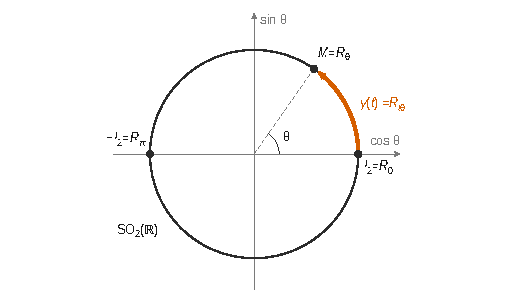
\includegraphics{figures/q4-chemin-so2.pdf}
\caption*{Figure 1 --- Question 4, cas n = 2 : SO\_2(ℝ) vu comme le cercle unité
(R\_θ ↔ (cos θ, sin θ)) ; le chemin γ(t) = R\_tθ, t allant de 0 à 1,
relie I\_2 à M = R\_θ}
\end{figure}

\emph{Cas général.} On utilise le théorème de réduction des isométries en base orthonormée. Pour \(M\in{\mathrm{O}}_n(\mathbb R)\), il existe une matrice de passage \textbf{orthogonale} \(P\in{\mathrm{O}}_n(\mathbb R)\), qui dépend de \(M\), et des entiers \(r,s,q\) avec \(2r+s+q=n\), tels que

\equationajustee{M=P\,\mathrm{diag}\big(R_{\theta_1},\dots,R_{\theta_r},\underbrace{1,\dots,1}_{s},\underbrace{-1,\dots,-1}_{q}\big)\,P^\top.}

Rappel de preuve, par récurrence sur \(n\).

\(\chi_M\) a une racine \(\lambda\in\mathbb C\). Si \(\lambda\in\mathbb R\), un vecteur propre réel engendre une droite stable.

Sinon, \(\lambda=a+ib\) avec \(b\ne0\). Soit \(X=U+iV\) un vecteur propre associé, avec \(U,V\in\mathbb R^n\). En séparant parties réelle et imaginaire :

\equationajustee{\begin{aligned}MU&=aU-bV,\\MV&=bU+aV.\end{aligned}}

Le sous-espace \(\mathrm{Vect}(U,V)\) est donc stable. C'est bien un plan : si \(U,V\) étaient liés, \(U\) ou \(V\) serait un vecteur propre réel associé à \(\lambda\notin\mathbb R\).

Un sous-espace \(F\) stable par l'isométrie \(u\) vérifie \(u(F)=F\), car \(u\) est injective. Donc \(F^\perp\) est stable.

En effet, pour \(y\in F^\perp\) et \(z=u(z')\in F\), on a \(\langle u(y),z\rangle=\langle y,z'\rangle=0\).

On conclut avec Q2 (et sa remarque) sur les plans, et avec l'hypothèse de récurrence sur \(F^\perp\) ; la concaténation de bases orthonormées donne une matrice de passage orthogonale.

Si \(M\in{\mathrm{SO}}_n(\mathbb R)\), alors \(1=\det M=(-1)^q\), donc \(q\) est pair. Comme \(\mathrm{diag}(-1,-1)=R_\pi\), on regroupe les \(-1\) par paires :

\equationajustee{M=P\,\mathrm{diag}\big(R_{\theta_1},\dots,R_{\theta_k},1,\dots,1\big)\,P^\top .}

Pour \(t\in[0,1]\), posons

\equationajustee{\gamma(t)=P\,\mathrm{diag}\big(R_{t\theta_1},\dots,R_{t\theta_k},1,\dots,1\big)P^\top.}

Ce chemin est continu et à valeurs dans \({\mathrm{O}}_n(\mathbb R)\) (produit de matrices orthogonales). Son déterminant vaut \(\prod_j\det R_{t\theta_j}=1\). Il relie \(\gamma(0)=I_n\) à \(\gamma(1)=M\) dans \({\mathrm{SO}}_n(\mathbb R)\).

Deux éléments \(M,M'\) sont alors reliés en concaténant le chemin de \(M\) à \(I_n\) (parcouru à l'envers) et celui de \(I_n\) à \(M'\).

\equationajustee{\boxed{{\mathrm{SO}}_n(\mathbb R)\ \text{est connexe par arcs.}}}

\hypertarget{question-5}{%
\subsection{Question 5}\label{question-5}}

Si tout élément de \(H\) est de déterminant \(1\), alors \(H\subset{\mathrm{SO}}_n(\mathbb R)\), d'où \(H={\mathrm{SO}}_n(\mathbb R)\).

Sinon, soit \(A\in H\) avec \(\det A=-1\), et soit \(B\in{\mathrm{O}}_n(\mathbb R)\).

\begin{itemize}
\tightlist
\item
  Si \(\det B=1\), alors \(B\in{\mathrm{SO}}_n(\mathbb R)\subset H\).
\item
  Si \(\det B=-1\), posons \(C=A^{-1}B\), élément du groupe \({\mathrm{O}}_n(\mathbb R)\) de déterminant \(1\).
\end{itemize}

Donc \(C\in{\mathrm{SO}}_n(\mathbb R)\subset H\), puis \(B=AC\in H\), car \(H\) est stable par produit.

Ainsi \({\mathrm{O}}_n(\mathbb R)\subset H\subset{\mathrm{O}}_n(\mathbb R)\).

\equationajustee{\boxed{H={\mathrm{SO}}_n(\mathbb R)\ \text{ou}\ H={\mathrm{O}}_n(\mathbb R)}}

\hypertarget{question-6}{%
\subsection{Question 6}\label{question-6}}

\emph{\({\mathrm{GL}}_2\).} On a \(\det Z_2=U-V\) avec \(U=Y_{1,1}Y_{2,2}\) et \(V=Y_{1,2}Y_{2,1}\).

Les variables \(Y_{i,j}\) sont indépendantes. Par le lemme des coalitions, \(U\) et \(V\) sont indépendantes, et chacune suit la loi \(\mathcal B(p^2)\).

Comme \(U,V\in\{0,1\}\), on a \(\det Z_2=0\) si et seulement si \(U=V\). Par indépendance :

\equationajustee{\begin{aligned}
P(Z_2\notin{\mathrm{GL}}_2(\mathbb R))&=P(U=V=1)+P(U=V=0)\\
&=p^4+(1-p^2)^2.
\end{aligned}}

\equationajustee{\boxed{P(Z_2\in{\mathrm{GL}}_2(\mathbb R))=1-p^4-(1-p^2)^2=2p^2(1-p^2)}}

\emph{\({\mathrm{O}}_n\).} Soit \(A\) à coefficients dans \(\{0,1\}\) avec \(A^\top A=I_n\).

La colonne \(j\) vérifie \(\sum_ia_{ij}^2=\sum_ia_{ij}=1\) : elle contient exactement un \(1\), situé en ligne \(\sigma(j)\).

Pour \(j\ne j'\), le produit scalaire des colonnes \(j\) et \(j'\) est nul, ce qui interdit \(\sigma(j)=\sigma(j')\).

L'application \(\sigma\) est injective de \(\{1,\dots,n\}\) dans lui-même, donc bijective : chaque ligne contient aussi exactement un \(1\), et \(A\) est une matrice de permutation \(P_\sigma\).

Réciproquement, toute matrice de permutation est orthogonale : ses colonnes sont la base canonique permutée.

Il y a \(n!\) matrices de permutation. Chacune a \(n\) coefficients égaux à \(1\) et \(n^2-n\) coefficients nuls.

Par indépendance des \(Y_{i,j}\), chacune est atteinte avec probabilité \(p^n(1-p)^{n^2-n}\). Ces \(n!\) événements sont deux à deux incompatibles.

\equationajustee{\boxed{P(Z_n\in{\mathrm{O}}_n(\mathbb R))=n!\,p^n(1-p)^{n(n-1)}}}

\emph{\({\mathrm{SO}}_n\).} D'après ce qui précède, \(Z_n\in{\mathrm{SO}}_n(\mathbb R)\) si et seulement si \(Z_n=P_\sigma\) avec \(\det P_\sigma=\varepsilon(\sigma)=1\), c'est-à-dire \(\sigma\) paire.

Comme \(n\ge2\), la transposition \(\tau=(1\ 2)\) existe. L'application \(\sigma\mapsto\tau\sigma\) est une bijection de l'ensemble des permutations paires sur celui des permutations impaires (sa réciproque est \(\sigma\mapsto\tau\sigma\)). Il y a donc \(n!/2\) permutations paires, chacune de probabilité \(p^n(1-p)^{n^2-n}\).

\equationajustee{\boxed{P(Z_n\in{\mathrm{SO}}_n(\mathbb R))=\frac{n!}{2}\,p^n(1-p)^{n(n-1)}}}

\hypertarget{question-7}{%
\subsection{Question 7}\label{question-7}}

\emph{Cas \(x\ne y\).} Soit \(u=\dfrac{x-y}{\|x-y\|}\) et \(A=I_n-2uu^\top\).

Pour \(z\in E\), \(Az=z-2\langle u,z\rangle u\).

Donc \(A\) fixe tout vecteur de l'hyperplan \(u^\perp\) et envoie \(u\) sur \(-u\) : c'est la matrice de la réflexion d'hyperplan \(u^\perp\).

On note aussi que \(A^\top=A\) et \(A^2=I_n\).

L'hypothèse \(\|x\|=\|y\|\) donne l'orthogonalité de \(x-y\) et \(x+y\) :

\equationajustee{\langle x-y,x+y\rangle=\|x\|^2-\|y\|^2=0.}

Ainsi \(x+y\in u^\perp\), donc \(A(x+y)=x+y\), et \(A(x-y)=-(x-y)\). En faisant la demi-somme :

\equationajustee{\begin{aligned}
Ax&=\tfrac12\big(A(x+y)+A(x-y)\big)\\
&=\tfrac12\big((x+y)-(x-y)\big)\\
&=y.
\end{aligned}}

\emph{Cas \(x=y\).} L'identité n'est pas une réflexion. Comme \(n\ge2\), il existe \(v\) unitaire orthogonal à \(x\).

La réflexion \(A=I_n-2vv^\top\), d'hyperplan \(v^\perp\ni x\), vérifie \(Ax=x=y\).

\equationajustee{\boxed{\text{Il existe une \text{réflexion} }A\text{ telle que }Ax=y.}}

\begin{figure}[H]
\centering
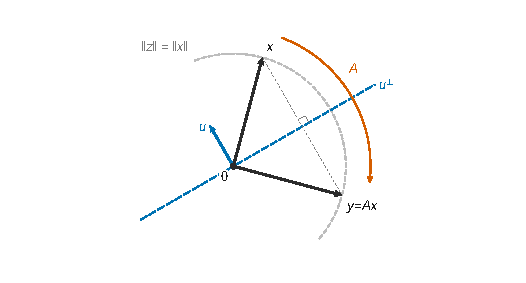
\includegraphics{figures/q7-reflexion.pdf}
\caption*{Figure 2 --- Question 7, dans le plan Vect(x, y) : la réflexion A
d'hyperplan u\^{}⊥, u = (x − y)/‖x − y‖, envoie x sur y ; u\^{}⊥ est
l'hyperplan médiateur du segment d'extrémités x et y}
\end{figure}

\hypertarget{question-8}{%
\subsection{Question 8}\label{question-8}}

Soit \(c=\|Gx\|\). Comme \(G\) est inversible et \(x\ne0\), on a \(c>0\).

\emph{\(p=1\).} Les vecteurs \(Gx\) et \(cx\) ont même norme \(c\). Par Q7, il existe une réflexion \(A\) telle que \(A(Gx)=cx\).

Or \(A\in{\mathrm{O}}_n(\mathbb R)\subset\mathcal G\) et \(\mathcal G\) est un groupe, donc \(G_1=AG\in\mathcal G\), et \(G_1x=cx\).

\emph{\(p\in\mathbb Z\).} Posons \(G_p=G_1^p\), qui appartient à \(\mathcal G\) (groupe). Par récurrence, \(G_1^px=c^px\) pour \(p\in\mathbb N\).

De \(G_1x=cx\) on tire \(G_1^{-1}x=c^{-1}x\), puis \(G_1^{-p}x=c^{-p}x\) par la même récurrence.

\equationajustee{\boxed{\forall p\in\mathbb Z,\ G_p=(AG)^p\in\mathcal G\ \text{ \text{vérifie} }\ G_px=\|Gx\|^p\,x.}}

\hypertarget{question-9}{%
\subsection{Question 9}\label{question-9}}

\(\mathcal G\) est compact et \(H\mapsto Hx\) est linéaire, donc continue. L'ensemble \(\{Hx,\ H\in\mathcal G\}\) est donc compact, et borné par un réel \(R>0\).

D'après Q8, \(c^p=\|G_px\|\le R\) pour tout \(p\in\mathbb Z\), avec \(c=\|Gx\|>0\).

\begin{itemize}
\tightlist
\item
  Si \(c>1\), \(c^p\to+\infty\) quand \(p\to+\infty\) : contradiction.
\item
  Si \(c<1\), \(c^p\to+\infty\) quand \(p\to-\infty\) : contradiction.
\end{itemize}

Donc \(\|Gx\|=1\) pour tout \(x\) unitaire, puis \(\|Gv\|=\|v\|\) pour tout \(v\in E\) par homogénéité.

Par polarisation, pour \(u,v\in E\) :

\equationajustee{\begin{aligned}
\langle Gu,Gv\rangle&=\tfrac12\big(\|G(u+v)\|^2-\|Gu\|^2-\|Gv\|^2\big)\\
&=\tfrac12\big(\|u+v\|^2-\|u\|^2-\|v\|^2\big)\\
&=\langle u,v\rangle.
\end{aligned}}

Ainsi \(\langle(G^\top G-I_n)u,v\rangle=0\) pour tous \(u,v\), soit \(G^\top G=I_n\). Donc \(\mathcal G\subset{\mathrm{O}}_n(\mathbb R)\), et l'inclusion inverse est une hypothèse.

\equationajustee{\boxed{\mathcal G={\mathrm{O}}_n(\mathbb R)}}

\begin{center}\rule{0.5\linewidth}{0.5pt}\end{center}

\hypertarget{ii.-calcul-diffuxe9rentiel-sur-mathrmo_nmathbb-r-et-mathrmsl_nmathbb-r}{%
\section{\texorpdfstring{II. Calcul différentiel sur \({\mathrm{O}}_n(\mathbb R)\) et \({\mathrm{SL}}_n(\mathbb R)\)}{II. Calcul différentiel sur \{\textbackslash mathrm\{O\}\}\_n(\textbackslash mathbb R) et \{\textbackslash mathrm\{SL\}\}\_n(\textbackslash mathbb R)}}\label{ii.-calcul-diffuxe9rentiel-sur-mathrmo_nmathbb-r-et-mathrmsl_nmathbb-r}}

\hypertarget{question-10}{%
\subsection{Question 10}\label{question-10}}

\emph{Classe \(\mathcal C^1\).} Chaque coordonnée de \(f\), à savoir \((M^\top M)_{ij}=\sum_km_{ki}m_{kj}\), est une fonction polynomiale des coefficients de \(M\).

Ses dérivées partielles existent et sont continues : \(f\) est \(\mathcal C^1\) (et même \(\mathcal C^\infty\)).

\emph{Différentielle.} Pour \(M,H\in\mathcal M_n(\mathbb R)\) :

\equationajustee{f(M+H)=M^\top M+(M^\top H+H^\top M)+H^\top H.}

L'application \(H\mapsto M^\top H+H^\top M\) est linéaire (la transposition et les produits à gauche et à droite le sont).

Le reste est négligeable. Le coefficient \((H^\top H)_{ij}\) est le produit scalaire des colonnes \(i\) et \(j\) de \(H\). Par Cauchy--Schwarz, \(|(H^\top H)_{ij}|\le\|H\|^2\). En sommant les \(n^2\) carrés :

\equationajustee{\|H^\top H\|\le n\|H\|^2=o(\|H\|).}

\equationajustee{\boxed{\mathrm df(M)(H)=M^\top H+H^\top M}}

\hypertarget{question-11}{%
\subsection{Question 11}\label{question-11}}

Soit \(H\in T\) et \(\gamma\) comme dans l'énoncé. Pour tout \(t\in\,]-\varepsilon,\varepsilon[\), on a \(\gamma(t)^\top\gamma(t)=I_n\).

L'application \((A,B)\mapsto A^\top B\) est bilinéaire. La fonction \(t\mapsto\gamma(t)^\top\gamma(t)\) est donc dérivable en \(0\), comme image de deux fonctions dérivables en \(0\) par une application bilinéaire. Sa dérivée en \(0\) vaut

\equationajustee{\gamma'(0)^\top\gamma(0)+\gamma(0)^\top\gamma'(0)=H^\top+H.}

Cette fonction étant constante, sa dérivée est nulle.

\equationajustee{\boxed{H^\top=-H,\quad\text{donc}\ T\subset\mathcal A_n(\mathbb R).}}

\hypertarget{question-12}{%
\subsection{Question 12}\label{question-12}}

\emph{\(T\) est non vide.} La matrice nulle appartient à \(T\) : le chemin constant égal à \(I_n\) est à valeurs dans \({\mathrm{O}}_n(\mathbb R)\) et de dérivée nulle en \(0\).

\emph{Somme.} Soient \(H,K\in T\), associés à \(\gamma\) (sur \(]-\varepsilon_1,\varepsilon_1[\)) et à \(\delta\) (sur \(]-\varepsilon_2,\varepsilon_2[\)). Soit \(\varepsilon=\min(\varepsilon_1,\varepsilon_2)\).

Sur \(]-\varepsilon,\varepsilon[\), posons \(\sigma(t)=\gamma(t)\delta(t)\). Comme \({\mathrm{O}}_n(\mathbb R)\) est un groupe, \(\sigma\) est à valeurs dans \({\mathrm{O}}_n(\mathbb R)\), et \(\sigma(0)=I_n\).

La dérivabilité en \(0\) donne les développements \(\gamma(t)=I_n+tH+o(t)\) et \(\delta(t)=I_n+tK+o(t)\). D'où

\equationajustee{\sigma(t)=I_n+t(H+K)+o(t).}

Ainsi \(\sigma\) est dérivable en \(0\), de dérivée \(H+K\) : \(H+K\in T\).

\emph{Produit par un scalaire.} Soit \(\lambda\ne0\). L'application \(t\mapsto\gamma(\lambda t)\) est définie sur \(]-\varepsilon/|\lambda|,\varepsilon/|\lambda|[\) et à valeurs dans \({\mathrm{O}}_n(\mathbb R)\).

Elle vaut \(I_n\) en \(0\) et a pour dérivée \(\lambda H\) en \(0\). Pour \(\lambda=0\), \(0\in T\).

\equationajustee{\boxed{T\ \text{est un sous-espace vectoriel de }\mathcal M_n(\mathbb R).}}

\hypertarget{question-13}{%
\subsection{Question 13}\label{question-13}}

Soit \(H\in\mathcal A_n(\mathbb R)\) et \(\gamma(t)=\exp(tH)\) pour \(t\in\mathbb R\).

Par continuité de la transposition sur les sommes partielles, \(\exp(tH)^\top=\exp(tH^\top)=\exp(-tH)\).

Les matrices \(tH\) et \(-tH=tH^\top\) commutent. Donc

\equationajustee{\begin{aligned}
\gamma(t)^\top\gamma(t)&=\exp(-tH)\exp(tH)\\
&=\exp(0)=I_n.
\end{aligned}}

\(\gamma\) est à valeurs dans \({\mathrm{O}}_n(\mathbb R)\). Elle est dérivable, de dérivée \(H\exp(tH)\), avec \(\gamma(0)=I_n\) et \(\gamma'(0)=H\). Donc \(\mathcal A_n(\mathbb R)\subset T\) et, avec Q11 :

\equationajustee{\boxed{T=\mathcal A_n(\mathbb R)}}

En particulier, \(\dim T=\dfrac{n(n-1)}{2}\).

\hypertarget{question-14}{%
\subsection{Question 14}\label{question-14}}

L'entier \(n\ge2\) est fixé. Pour \(t>0\), la matrice \(D_t=\mathrm{diag}(t,1/t,1,\dots,1)\) est de déterminant \(1\), donc dans \({\mathrm{SL}}_n(\mathbb R)\). Et

\equationajustee{g(D_t)=t^2+\frac1{t^2}+n-2\xrightarrow[t\to+\infty]{}+\infty.}

\equationajustee{\boxed{g_{|{\mathrm{SL}}_n(\mathbb R)}\ \text{n'est pas \text{majorée}, donc n'a pas de maximum global.}}}

\hypertarget{question-15}{%
\subsection{Question 15}\label{question-15}}

\(g(M)=\sum_{i,j}m_{ij}^2\) et \(\det M=\sum_{\sigma\in\mathfrak S_n}\varepsilon(\sigma)\prod_im_{\sigma(i)i}\) sont des fonctions polynomiales des coefficients de \(M\). Leurs dérivées partielles existent et sont continues : elles sont \(\mathcal C^1\).

Les gradients sont pris pour le produit scalaire \(\langle A,B\rangle=\mathrm{tr}(A^\top B)\).

\emph{Gradient de \(g\).} Comme \(\mathrm{tr}(H^\top M)=\mathrm{tr}(M^\top H)\),

\equationajustee{g(M+H)=g(M)+2\,\mathrm{tr}(M^\top H)+\|H\|^2,}

avec \(\|H\|^2=o(\|H\|)\). Donc \(\mathrm dg(M)(H)=\langle2M,H\rangle\).

\emph{Gradient de \(\det\).} Notons \(\Delta_{ij}\) le mineur d'indice \((i,j)\) : le déterminant de la matrice extraite en supprimant la ligne \(i\) et la colonne \(j\).

Le cofacteur est \(c_{ij}=(-1)^{i+j}\Delta_{ij}\), et \(\mathrm{Com}(M)=(c_{ij})\).

Développons \(\det M\) selon la ligne \(i\) : \(\det M=\sum_km_{ik}c_{ik}\). Aucun cofacteur \(c_{ik}\) ne dépend des coefficients de la ligne \(i\). Donc \(\dfrac{\partial\det}{\partial m_{ij}}(M)=c_{ij}\).

Comme \(\det\) est \(\mathcal C^1\), sa différentielle s'exprime avec les dérivées partielles :

\equationajustee{\begin{aligned}
\mathrm d\det(M)(H)&=\sum_{i,j}c_{ij}h_{ij}\\
&=\mathrm{tr}\big(\mathrm{Com}(M)^\top H\big)\\
&=\langle\mathrm{Com}(M),H\rangle.
\end{aligned}}

\equationajustee{\boxed{\nabla g(M)=2M}}

\equationajustee{\boxed{\nabla\det(M)=\mathrm{Com}(M)}}

\hypertarget{question-16}{%
\subsection{Question 16}\label{question-16}}

On utilise le théorème d'optimisation sous une contrainte, que l'on énonce.

\emph{Soient \(U\) un ouvert de \(\mathbb R^d\) et \(\phi,h:U\to\mathbb R\) deux fonctions de classe \(\mathcal C^1\).}

\emph{On pose \(X=h^{-1}(\{0\})\).}

\emph{Si \(\phi_{|X}\) admet un extremum local en \(a\in X\) et si \(\mathrm dh(a)\ne0\), alors \(\mathrm d\phi(a)\) est colinéaire à \(\mathrm dh(a)\).}

\emph{Vérification des hypothèses.} L'ouvert est \(\mathcal M_n(\mathbb R)\), identifié à \(\mathbb R^{n^2}\). Les fonctions \(g\) et \(h=\det-1\) sont \(\mathcal C^1\) (Q15). Et \({\mathrm{SL}}_n(\mathbb R)=h^{-1}(\{0\})\).

En \(M\in{\mathrm{SL}}_n(\mathbb R)\), on a \(M\,\mathrm{Com}(M)^\top=\det(M)I_n=I_n\). Donc \(\mathrm{Com}(M)^\top=M^{-1}\) est inversible. En particulier \(\nabla h(M)=\mathrm{Com}(M)\ne0\), c'est-à-dire \(\mathrm dh(M)\ne0\).

\emph{Conclusion.} Si \(g_{|{\mathrm{SL}}_n(\mathbb R)}\) a un extremum local en \(M\), \(\mathrm dg(M)\) est colinéaire à \(\mathrm dh(M)\).

Il existe donc \(\mu\in\mathbb R\) tel que \(2M=\mu\,\mathrm{Com}(M)\). On pose \(\lambda=\mu/2\).

\equationajustee{\boxed{\exists\lambda\in\mathbb R,\quad M=\lambda\,\mathrm{Com}(M).}}

Alors \(M^\top=\lambda\,\mathrm{Com}(M)^\top=\lambda M^{-1}\), donc \(M^\top M=\lambda I_n\).

\begin{itemize}
\tightlist
\item
  En prenant la trace : \(n\lambda=\|M\|^2>0\), donc \(\lambda>0\).
\item
  En prenant le déterminant : \(\lambda^n=\det(\lambda I_n)=\det(M)^2=1\).
\end{itemize}

Le réel \(\lambda>0\) vérifie \(\lambda^n=1\), donc \(\lambda=1\). Ainsi \(M^\top M=I_n\) et \(\det M=1\).

\equationajustee{\boxed{M\in{\mathrm{SO}}_n(\mathbb R)}}

\hypertarget{question-17}{%
\subsection{Question 17}\label{question-17}}

\emph{Existence.} Soit \(K=\{M\in{\mathrm{SL}}_n(\mathbb R),\ g(M)\le n\}\).

\begin{itemize}
\tightlist
\item
  \(K\) contient \(I_n\), car \(g(I_n)=n\).
\item
  \(K\) est fermé : c'est l'intersection de \(\det^{-1}(\{1\})\) et de \(g^{-1}(]-\infty,n])\), images réciproques de fermés par des applications continues.
\item
  \(K\) est borné : \(\|M\|\le\sqrt n\) sur \(K\).
\end{itemize}

\(K\) est donc une partie compacte non vide. La fonction continue \(g\) y atteint son minimum en un point \(M_0\).

Pour \(M\in{\mathrm{SL}}_n(\mathbb R)\setminus K\), on a \(g(M)>n=g(I_n)\ge g(M_0)\). Donc \(M_0\) est un minimum global de \(g\) sur \({\mathrm{SL}}_n(\mathbb R)\).

\emph{Valeur et points.} Tout point de minimum global est un extremum local. D'après Q16, il appartient à \({\mathrm{SO}}_n(\mathbb R)\), où \(g(M)=\mathrm{tr}(I_n)=n\).

Réciproquement, tout \(M\in{\mathrm{SO}}_n(\mathbb R)\) est dans \({\mathrm{SL}}_n(\mathbb R)\) avec \(g(M)=n\).

\equationajustee{\boxed{\min_{{\mathrm{SL}}_n(\mathbb R)}g=n,\ \text{atteint exactement sur }{\mathrm{SO}}_n(\mathbb R).}}

\begin{figure}[H]
\centering
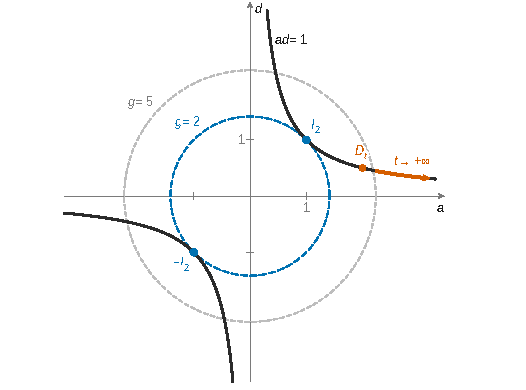
\includegraphics{figures/q14-q17-tranche-diagonale.pdf}
\caption*{Figure 3 --- Questions 14 et 17, cas n = 2, matrices diagonales diag(a,
d) : contrainte ad = 1 et lignes de niveau a² + d² = g ; le minimum g =
2 est atteint en ±I\_2, et D\_t = diag(t, 1/t) part à l'infini}
\end{figure}

\begin{center}\rule{0.5\linewidth}{0.5pt}\end{center}

\hypertarget{iii.-morphismes-continus-de-mathbb-u-dans-mathrmgl_nmathbb-r}{%
\section{\texorpdfstring{III. Morphismes continus de \(\mathbb U\) dans \({\mathrm{GL}}_n(\mathbb R)\)}{III. Morphismes continus de \textbackslash mathbb U dans \{\textbackslash mathrm\{GL\}\}\_n(\textbackslash mathbb R)}}\label{iii.-morphismes-continus-de-mathbb-u-dans-mathrmgl_nmathbb-r}}

\hypertarget{question-18}{%
\subsection{Question 18}\label{question-18}}

\emph{Sous-groupes bornés de \(\mathbb R^*\).} Soit \(H\) un tel sous-groupe et \(x\in H\). Alors \(x^k\in H\) pour tout \(k\in\mathbb Z\), donc la famille \((|x|^k)_{k\in\mathbb Z}\) est bornée.

\begin{itemize}
\tightlist
\item
  Si \(|x|>1\), \(|x|^k\to+\infty\) quand \(k\to+\infty\) : contradiction.
\item
  Si \(|x|<1\), \(|x|^k\to+\infty\) quand \(k\to-\infty\) : contradiction.
\end{itemize}

Donc \(|x|=1\), et \(H\subset\{-1,1\}\). Comme \(1\in H\), \(H\) vaut \(\{1\}\) ou \(\{-1,1\}\). Réciproquement, ces deux ensembles sont des sous-groupes bornés.

\equationajustee{\boxed{\text{Les sous-groupes \text{bornés} de }(\mathbb R^*,\times)\text{ sont }\{1\}\text{ et }\{-1,1\}.}}

\emph{Conséquence.} L'application \(\det\circ\varphi:\mathbb U\to\mathbb R^*\) est un morphisme continu. Son image est un sous-groupe de \(\mathbb R^*\). Elle est compacte, comme image continue du compact \(\mathbb U\), donc bornée. Elle est donc contenue dans \(\{-1,1\}\).

\(\mathbb U\) est connexe par arcs, paramétré par \(\theta\mapsto e^{i\theta}\). La fonction continue \(\theta\mapsto\det\varphi(e^{i\theta})\) est définie sur l'intervalle \(\mathbb R\).

Elle vaut \(\det\varphi(1)=\det I_n=1\) en \(0\). Si elle valait \(-1\) en un point, elle s'annulerait par le théorème des valeurs intermédiaires. C'est exclu, car \(\varphi(e^{i\theta})\in{\mathrm{GL}}_n(\mathbb R)\). Donc \(\det\varphi(z)=1\) pour tout \(z\in\mathbb U\).

\equationajustee{\boxed{\varphi(\mathbb U)\subset{\mathrm{SL}}_n(\mathbb R)}}

\hypertarget{question-19}{%
\subsection{Question 19}\label{question-19}}

Soit \(\lambda\in{\mathrm{Sp}}_{\mathbb C}(\varphi(z))\) et \(X\in\mathbb C^n\setminus\{0\}\) avec \(\varphi(z)X=\lambda X\). On a \(\lambda\ne0\), car \(\varphi(z)\) est inversible.

Pour \(k\in\mathbb Z\), \(\varphi(z^k)=\varphi(z)^k\) (morphisme), et \(\varphi(z)^kX=\lambda^kX\).

L'ensemble \(\varphi(\mathbb U)\) est compact (image continue d'un compact), et \(A\mapsto AX\) est continue. Il existe donc \(R\) tel que \(\|AX\|\le R\) pour tout \(A\in\varphi(\mathbb U)\), pour la norme hermitienne de \(\mathbb C^n\).

Ainsi \(|\lambda|^k\|X\|\le R\) pour tout \(k\in\mathbb Z\). Comme en Q18, cela impose \(|\lambda|=1\).

\equationajustee{\boxed{{\mathrm{Sp}}_{\mathbb C}(\varphi(z))\subset\mathbb U}}

\hypertarget{question-20}{%
\subsection{Question 20}\label{question-20}}

Comme \(\varphi\) est un morphisme de groupes :

\equationajustee{\Psi(x+y)=\varphi(e^{ix}e^{iy})=\varphi(e^{ix})\varphi(e^{iy}).}

\equationajustee{\boxed{\forall(x,y)\in\mathbb R^2,\ \Psi(x+y)=\Psi(x)\Psi(y)}}

De plus, \(\Psi\) est continue (composée), \(\Psi(0)=\varphi(1)=I_n\), et \(\Psi\) est \(2\pi\)-périodique.

\hypertarget{question-21}{%
\subsection{Question 21}\label{question-21}}

\(\Psi\) est continue sur \(\mathbb R\), à valeurs dans l'espace de dimension finie \(\mathcal M_n(\mathbb R)\).

Par le théorème fondamental de l'analyse, \(F\) est la primitive de \(\Psi\) nulle en \(0\) : \(F\) est dérivable, de dérivée \(\Psi\) continue.

Donc \(F\) est \(\mathcal C^1\), avec \(F(0)=0\) et \(F'(0)=I_n\).

\({\mathrm{GL}}_n(\mathbb R)=\det^{-1}(\mathbb R^*)\) est ouvert, image réciproque de l'ouvert \(\mathbb R^*\) par l'application continue \(\det\). Il existe donc \(r>0\) tel que \(\|A-I_n\|<r\) entraîne \(A\in{\mathrm{GL}}_n(\mathbb R)\).

Comme \(F(x)/x\to F'(0)=I_n\) quand \(x\to0\), il existe \(\alpha>0\) tel que, pour \(0<|x|\le\alpha\), \(\|F(x)/x-I_n\|<r\).

Pour ces \(x\), \(F(x)/x\) est inversible, donc \(F(x)=x\cdot\frac{F(x)}x\) aussi (\(x\ne0\)).

\equationajustee{\boxed{F\in\mathcal C^1(\mathbb R),\quad\exists\alpha>0,\ \forall x\in[-\alpha,\alpha]\setminus\{0\},\ F(x)\in{\mathrm{GL}}_n(\mathbb R).}}

\hypertarget{question-22}{%
\subsection{Question 22}\label{question-22}}

On fait le changement de variable \(t=x+s\), puis on utilise Q20 et la linéarité de l'intégrale vis-à-vis de l'application linéaire \(A\mapsto\Psi(x)A\). Le facteur \(\Psi(x)\) reste \textbf{à gauche} :

\equationajustee{\begin{aligned}
\int_x^{x+\alpha}\Psi(t)\,\mathrm dt&=\int_0^\alpha\Psi(x)\Psi(s)\,\mathrm ds\\
&=\Psi(x)F(\alpha).
\end{aligned}}

\(F(\alpha)\) est inversible (Q21). En multipliant à droite par \(F(\alpha)^{-1}\) et avec la relation de Chasles :

\equationajustee{\boxed{\Psi(x)=\left(\int_x^{x+\alpha}\Psi(t)\,\mathrm dt\right)F(\alpha)^{-1}=\big(F(x+\alpha)-F(x)\big)F(\alpha)^{-1}.}}

Le membre de droite est \(\mathcal C^1\), car \(F\) l'est et \(A\mapsto AF(\alpha)^{-1}\) est linéaire. \textbf{\(\Psi\) est de classe \(\mathcal C^1\) sur \(\mathbb R\).}

\hypertarget{question-23}{%
\subsection{Question 23}\label{question-23}}

Pour \(x\in\mathbb R\) et \(h\ne0\), Q20 donne

\equationajustee{\frac{\Psi(x+h)-\Psi(x)}h=\Psi(x)\,\frac{\Psi(h)-I_n}h\xrightarrow[h\to0]{}\Psi(x)M,}

car \(\Psi(0)=I_n\) et \(M=\Psi'(0)\). Donc \(\Psi'=\Psi M\), dans cet ordre.

Soit \(\Theta(x)=\Psi(x)\exp(-xM)\). L'application \(x\mapsto\exp(-xM)\) est dérivable de dérivée \(-M\exp(-xM)\). Par dérivation d'un produit :

\equationajustee{\begin{aligned}
\Theta'(x)&=\Psi(x)M\exp(-xM)-\Psi(x)M\exp(-xM)\\
&=0.
\end{aligned}}

\(\Theta\) est constante sur l'intervalle \(\mathbb R\), égale à \(\Theta(0)=I_n\). On multiplie à droite par \(\exp(xM)=\exp(-xM)^{-1}\) :

\equationajustee{\boxed{\forall x\in\mathbb R,\ \Psi(x)=\varphi(e^{ix})=\exp(xM).}}

\begin{center}\rule{0.5\linewidth}{0.5pt}\end{center}

\hypertarget{iv.-morphismes-de-mathbb-r-dans-mathrmgl_nmathbb-rtimes}{%
\section{\texorpdfstring{IV. Morphismes de \((\mathbb R,+)\) dans \(({\mathrm{GL}}_n(\mathbb R),\times)\)}{IV. Morphismes de (\textbackslash mathbb R,+) dans (\{\textbackslash mathrm\{GL\}\}\_n(\textbackslash mathbb R),\textbackslash times)}}\label{iv.-morphismes-de-mathbb-r-dans-mathrmgl_nmathbb-rtimes}}

\hypertarget{question-24}{%
\subsection{Question 24}\label{question-24}}

Soit \(P\in{\mathrm{GL}}_n(\mathbb C)\) avec \(AP=PB\). Écrivons \(P=R+iS\) avec \(R,S\in\mathcal M_n(\mathbb R)\).

Comme \(A\) et \(B\) sont réelles, l'identification des parties réelle et imaginaire donne \(AR=RB\) et \(AS=SB\). Donc \(A(R+tS)=(R+tS)B\) pour tout \(t\).

La fonction \(\pi:t\mapsto\det(R+tS)\) est polynomiale, de degré au plus \(n\), à coefficients réels. Évaluée en \(i\), elle vaut \(\pi(i)=\det P\ne0\).

\(\pi\) n'est donc pas le polynôme nul : elle n'a qu'un nombre fini de racines. Il existe ainsi \(t_0\in\mathbb R\) avec \(\pi(t_0)\ne0\).

La matrice \(Q=R+t_0S\) est réelle, inversible, et vérifie \(AQ=QB\).

\equationajustee{\boxed{A=QBQ^{-1}\ \text{avec}\ Q\in{\mathrm{GL}}_n(\mathbb R).}}

\hypertarget{question-25}{%
\subsection{Question 25}\label{question-25}}

On a toujours \(\ker N\subset\ker N^2\).

Soit \(r\ge1\) l'indice de nilpotence de \(N\), c'est-à-dire le plus petit entier tel que \(N^r=0\). Comme \(N\ne0\), \(r\ge2\).

Par minimalité, \(N^{r-1}\ne0\) : soit \(x\) tel que \(N^{r-1}x\ne0\), et \(y=N^{r-2}x\).

Alors \(N^2y=N^rx=0\) et \(Ny=N^{r-1}x\ne0\). Donc \(y\in\ker N^2\setminus\ker N\).

\equationajustee{\boxed{\ker N\ne\ker N^2}}

\hypertarget{question-26}{%
\subsection{Question 26}\label{question-26}}

Par Q23, \(\exp(2\pi M)=\Psi(2\pi)=\varphi(e^{2i\pi})=\varphi(1)=I_n\).

Soit \(X\in\mathbb C^n\setminus\{0\}\) avec \(MX=\lambda X\). Alors \(M^kX=\lambda^kX\) pour tout \(k\). Par passage à la limite dans les sommes partielles, \(\exp(2\pi M)X=e^{2\pi\lambda}X\).

Donc \(e^{2\pi\lambda}X=X\) avec \(X\ne0\), soit \(e^{2\pi\lambda}=1\). Cela donne \(2\pi\lambda\in2i\pi\mathbb Z\), c'est-à-dire \(\lambda\in i\mathbb Z\).

\equationajustee{\boxed{\exp(2\pi M)=I_n}}

\equationajustee{\boxed{{\mathrm{Sp}}_{\mathbb C}(M)\subset\{ik,\ k\in\mathbb Z\}}}

\hypertarget{question-27}{%
\subsection{Question 27}\label{question-27}}

Sur \(\mathbb C\), le polynôme caractéristique est scindé : \(\chi_M=\prod_{j=1}^r(X-\lambda_j)^{m_j}\), les \(\lambda_j\) étant distinctes.

Par le théorème de Cayley--Hamilton et le lemme des noyaux, \(\mathbb C^n=\bigoplus_jF_j\), où \(F_j=\ker(M-\lambda_jI_n)^{m_j}\) est le sous-espace caractéristique associé à \(\lambda_j\). Chaque \(F_j\) est stable par \(M\) et de dimension \(m_j\).

Sur \(F_j\), l'endomorphisme induit s'écrit \(\lambda_j\mathrm{id}+\nu_j\), avec \(\nu_j^{m_j}=0\) par définition de \(F_j\).

Dans une base adaptée à cette décomposition, de matrice de passage \(P\in{\mathrm{GL}}_n(\mathbb C)\), la matrice de \(M\) est diagonale par blocs :

\equationajustee{P^{-1}MP=\mathrm{diag}\big(\lambda_1I_{m_1}+N_1,\dots,\lambda_rI_{m_r}+N_r\big),\quad N_j\ \text{nilpotente}.}

Posons \(D=\mathrm{diag}(\lambda_1I_{m_1},\dots,\lambda_rI_{m_r})\) et \(N=\mathrm{diag}(N_1,\dots,N_r)\).

\begin{itemize}
\tightlist
\item
  \(D\) est diagonale, et \({\mathrm{Sp}}_{\mathbb C}(D)=\{\lambda_1,\allowbreak \dots,\allowbreak \lambda_r\}={\mathrm{Sp}}_{\mathbb C}(M)\).
\item
  \(N^k=\mathrm{diag}(N_1^k,\dots,N_r^k)=0\) pour \(k\ge\max m_j\) : \(N\) est nilpotente.
\item
  \(DN=ND\), en calculant bloc par bloc, car chaque bloc de \(D\) est scalaire.
\end{itemize}

\equationajustee{\boxed{M=P(D+N)P^{-1},\ \text{avec}\ D\ \text{diagonale},\ N\ \text{nilpotente}\ \text{et}\ DN=ND.}}

De plus, \({\mathrm{Sp}}_{\mathbb C}(D)={\mathrm{Sp}}_{\mathbb C}(M)\).

\hypertarget{question-28}{%
\subsection{Question 28}\label{question-28}}

Les coefficients diagonaux \(\mu_1,\dots,\mu_n\) de \(D\) sont dans \({\mathrm{Sp}}_{\mathbb C}(M)\subset i\mathbb Z\). Donc

\equationajustee{\exp(2\pi D)=\mathrm{diag}\big(e^{2\pi\mu_1},\dots,e^{2\pi\mu_n}\big)=I_n.}

Pour \(P\) inversible, \(\exp(PAP^{-1})=P\exp(A)P^{-1}\) : l'égalité vaut pour les sommes partielles, et \(A\mapsto PAP^{-1}\) est continue. Par ailleurs \(D\) et \(N\) commutent, donc \(\exp(2\pi(D+N))=\exp(2\pi D)\exp(2\pi N)\). D'où

\equationajustee{\begin{aligned}
I_n=\exp(2\pi M)&=P\exp(2\pi D)\exp(2\pi N)P^{-1}\\
&=P\exp(2\pi N)P^{-1}.
\end{aligned}}

\equationajustee{\boxed{\exp(2\pi D)=I_n}}

\equationajustee{\boxed{\exp(2\pi N)=I_n}}

\(N\) étant nilpotente, la série de \(\exp(2\pi N)\) est une somme finie, et

\equationajustee{0=\exp(2\pi N)-I_n=2\pi N+N^2T,}

avec \(T=\sum_{k\ge2}\frac{(2\pi)^k}{k!}N^{k-2}\) (somme finie), polynôme en \(N\) qui commute donc avec \(N^2\).

Si \(N\ne0\), Q25 fournit \(y\in\ker N^2\setminus\ker N\). Alors \(2\pi Ny=-TN^2y=0\), ce qui contredit \(Ny\ne0\).

\equationajustee{\boxed{N=0\ :\ M\ \text{est diagonalisable dans }\mathcal M_n(\mathbb C).}}

\hypertarget{question-29}{%
\subsection{Question 29}\label{question-29}}

\(M\) est diagonalisable sur \(\mathbb C\), de spectre inclus dans \(i\mathbb Z\).

Comme \(M\) est réelle, \(\chi_M\in\mathbb R[X]\), donc \(ik\) et \(-ik\) ont la même multiplicité.

Notons \(k_1,\dots,k_p\in\mathbb N^*\) les entiers \(k>0\) tels que \(ik\in{\mathrm{Sp}}_{\mathbb C}(M)\), chacun répété selon sa multiplicité. La multiplicité de \(0\) est \(m_0=n-2p\), et

\equationajustee{\chi_M=X^{m_0}\prod_{j=1}^p(X^2+k_j^2).}

Soit \(J=\begin{pmatrix}0&-1\\1&0\end{pmatrix}\) et \(B=\mathrm{diag}(k_1J,\allowbreak \dots,\allowbreak k_pJ,\allowbreak 0,\allowbreak \dots,\allowbreak 0)\in\mathcal M_n(\mathbb R)\).

Chaque bloc \(k_jJ\) a deux valeurs propres distinctes \(\pm ik_j\), donc \(B\) est diagonalisable sur \(\mathbb C\), et \(\chi_B=\chi_M\).

Deux matrices diagonalisables de même polynôme caractéristique sont semblables à la même matrice diagonale. Donc \(M\) et \(B\) sont semblables dans \(\mathcal M_n(\mathbb C)\), puis dans \(\mathcal M_n(\mathbb R)\) par Q24 : \(M=QBQ^{-1}\) avec \(Q\in{\mathrm{GL}}_n(\mathbb R)\).

\textbf{La matrice \(Q\) ne dépend que de \(M\), donc pas de \(x\).} Pour tout \(x\in\mathbb R\), \(xM=Q(xB)Q^{-1}\), et, comme en Q28,

\equationajustee{\exp(xM)=Q\exp(xB)Q^{-1}.}

Comme \(J^2=-I_2\), en séparant les puissances paires et impaires :

\equationajustee{\begin{aligned}
\exp(\theta J)&=\Big(\sum_m\frac{(-1)^m\theta^{2m}}{(2m)!}\Big)I_2+\Big(\sum_m\frac{(-1)^m\theta^{2m+1}}{(2m+1)!}\Big)J\\
&=\cos(\theta)I_2+\sin(\theta)J\\
&=R_\theta.
\end{aligned}}

L'exponentielle d'une matrice diagonale par blocs se calcule bloc par bloc. On a donc \(\exp(xB)=\mathrm{diag}(R_{xk_1},\dots,R_{xk_p},1,\dots,1)\), et, avec Q23 :

\equationajustee{\boxed{\forall x\in\mathbb R,\ \Psi(x)=Q\,\mathrm{diag}\big(R_{xk_1},\dots,R_{xk_p},1,\dots,1\big)\,Q^{-1},\ \text{avec}\ Q\in{\mathrm{GL}}_n(\mathbb R),\ p\in\mathbb N,\ k_j\in\mathbb Z\setminus\{0\}.}}

\hypertarget{question-30}{%
\subsection{Question 30}\label{question-30}}

Soient \(Q\in{\mathrm{GL}}_n(\mathbb R)\), \(p\in\mathbb N\) avec \(2p\le n\), et \(k_1,\dots,k_p\in\mathbb Z\setminus\{0\}\). Posons \(B(x)=\mathrm{diag}(R_{xk_1},\dots,R_{xk_p},1,\dots,1)\) et \(\Psi(x)=QB(x)Q^{-1}\).

\emph{Valeurs.} \(\det\Psi(x)=\det B(x)=\prod_j\det R_{xk_j}=1\), donc \(\Psi(x)\in{\mathrm{GL}}_n(\mathbb R)\).

\emph{Morphisme.} Les formules d'addition donnent \(R_\theta R_{\theta'}=R_{\theta+\theta'}\). Le produit de matrices diagonales par blocs de même découpage se fait bloc par bloc, donc \(B(x)B(y)=B(x+y)\). Puis

\equationajustee{\begin{aligned}
\Psi(x)\Psi(y)&=QB(x)Q^{-1}QB(y)Q^{-1}\\
&=QB(x+y)Q^{-1}\\
&=\Psi(x+y).
\end{aligned}}

\equationajustee{\boxed{\Psi\ \text{est un morphisme de groupes de }(\mathbb R,+)\ \text{dans}\ ({\mathrm{GL}}_n(\mathbb R),\times).}}

\emph{Remarque.} Comme \(k_j\in\mathbb Z\), \(\Psi\) est \(2\pi\)-périodique. L'application \(\phi(e^{ix})=\Psi(x)\) est donc bien définie sur \(\mathbb U\), et c'est un morphisme.

Il est continu. Près de \(z_0=e^{ix_0}\), on a \(\phi(z)=\Psi\big(x_0+\mathrm{Arg}(z/z_0)\big)\), où \(\mathrm{Arg}(w)=2\arctan\dfrac{\mathrm{Im}\,w}{1+\mathrm{Re}\,w}\) est continue sur \(\mathbb U\setminus\{-1\}\).

Les questions 29 et 30 décrivent donc exactement les morphismes continus de \(\mathbb U\) dans \({\mathrm{GL}}_n(\mathbb R)\).

\end{document}
